%==============================================================================
%  RELATÓRIO 1  —  Entregue em 24/03/2026
%==============================================================================

\section{Relatório 1: Caracterização da Empresa e do Problema}

\subsection{Sobre a Empresa}

A Rentex é uma empresa do setor têxtil fundada em 1991, com sede na Rua João
Antônio de Oliveira, 1083, no bairro de Mooca/Belenzinho, São Paulo
(CEP 03111-001). Com cerca de 30 funcionários distribuídos em dois turnos, opera
no segmento B2B fabricando tecidos planos para confecção e uniformes. O contato
institucional para este projeto é Pedro Charmillot Silva, Diretor de Novos
Negócios, cuja autorização de uso da empresa para fins acadêmicos encontra-se
no Anexo~A.

A empresa é especializada em sarjas e forros, atendendo fabricantes de vestuário
que demandam materiais com composições específicas de algodão, poliéster e
elastano. Seu modelo comercial é baseado em parcerias de longo prazo: parte da
produção é comprometida semanalmente com clientes fixos por contrato.

\subsubsection{Portfólio de Produtos}

O portfólio ativo compreende quatro famílias:

\textbf{Sarja Barcelos (100\% algodão)} é o produto de maior volume da linha,
com processo mais padronizado e tempo de setup reduzido nos teares. Atende
principalmente confecção básica e uniformes. Sua margem unitária é a menor entre
as sarjas.

\textbf{Sarja Joy (mista poliéster/elastano)} tem composição aproximada de
70\% algodão, 25\% poliéster e 5\% elastano, o que exige troca de urdume e
trama nos teares a cada novo lote. O tempo de setup é significativamente maior,
mas a margem de contribuição compensa.

\textbf{Forro de Poliéster Padrão (100\% poliéster)} é um forro leve de
acabamento padronizado usado no interior de roupas e bolsas. Processo rápido,
alto volume, menor margem. Três clientes têm contrato de fornecimento mínimo
semanal para este produto.

\textbf{Forro de Poliéster Premium (95\% poliéster/5\% elastano)} é a variação
de maior valor do forro padrão, com acabamento acetinado voltado ao segmento de
moda feminina. Um cliente estratégico tem contrato de mínimo semanal.

\subsection{Definição do Problema}

Com cinco teares planos e armazenamento limitado de matéria-prima, a Rentex não
consegue atender simultaneamente toda a demanda de mercado de todos os produtos.
Toda semana o gerente de produção decide quanto produzir de cada tecido, e essa
decisão tem impacto direto no resultado financeiro.

O conflito central está entre os forros e as sarjas. Os forros têm alta demanda
e processo rápido, mas margem baixa, e parte da produção é obrigatória por
contrato. As sarjas têm setup mais demorado e menor demanda, mas margem
substancialmente maior. Produzir mais forro do que o necessário consome horas de
tear que poderiam gerar receita maior nas sarjas; produzir exclusivamente sarjas
significaria quebrar contratos com clientes de longo prazo.

O problema é, portanto, determinar o mix semanal que maximize a margem de
contribuição total sujeita às restrições de capacidade dos teares, de estoque
de matéria-prima, de mão de obra e de demanda.

\subsection{Concepção da Modelagem}

O problema se enquadra naturalmente em um modelo de Programação Linear. A
variável de decisão $x_j$ representa a quantidade de lotes de 100 metros do
produto $j$ a produzir por semana. A função objetivo maximiza a soma das margens
de contribuição, calculadas como preço de venda menos custos variáveis diretos
de cada produto.

Os parâmetros do modelo incluem os tempos de ciclo dos teares (com setup
amortizado sobre o tamanho mínimo de lote contratual), os coeficientes de
consumo de cada matéria-prima por lote e a disponibilidade semanal de cada
recurso, calculada a partir dos dois turnos de trabalho menos paradas programadas.

As restrições são de cinco tipos. A capacidade dos teares limita o total de
horas de máquina utilizadas por semana. Os estoques de algodão, poliéster e
elastano impõem limites ao consumo de cada insumo. A mão de obra disponível
dos 30 funcionários restringe as horas-homem semanais, mesmo com margem para
horas extras dentro dos limites da convenção coletiva. Os contratos de
fornecimento impõem quantidades mínimas semanais para os dois forros. Por fim,
os limites de demanda máxima de mercado definem o teto de produção para cada
família.

\subsection{Viabilidade do Projeto}

Os dados necessários para a formulação estão disponíveis no sistema de gestão
da empresa: roteiros de fabricação, relatórios de capacidade, fichas de custo e
histórico de pedidos. A Rentex confirmou, por intermédio de Pedro Charmillot
Silva, a disponibilidade de acesso a essas informações durante o desenvolvimento
do projeto. A formulação matemática completa e os primeiros resultados
computacionais serão apresentados no Relatório~2.

\subsection{Artigo de Referência}

O artigo selecionado é:

\begin{quote}
SOBREIRO, V. A.; NAGANO, M. S. Proposta de uma heurística construtiva baseada
na TOC para definição de mix de produção. \textit{Produção}, v.~23, n.~3,
p.~468--477, jul./set. 2013.
\end{quote}

O artigo aborda o mesmo problema estrutural da Rentex: múltiplos produtos
competindo por recursos produtivos insuficientes para atender toda a demanda,
com objetivo de maximizar o ganho total. Os autores utilizam a solução ótima
da Programação Linear Inteira como referência de qualidade e propõem heurísticas
construtivas baseadas na Teoria das Restrições para instâncias de maior escala.
A conexão com a metodologia adotada neste projeto é discutida em detalhe no
Relatório~2. O artigo completo encontra-se no Anexo~B.

\newpage

\subsection*{Anexo A -- Autorização da Empresa}

\begin{figure}[H]
\centering

\includegraphics[width=0.80\textwidth]{relatorio1/carta_empresa.pdf}
\caption{Autorização emitida pela Rentex Indústria Têxtil LTDA, contendo nome,
         cargo e telefone de contato do responsável, Pedro Charmillot Silva,
         Diretor de Novos Negócios (+55~11~99858-1812).}
\end{figure}

\newpage

\subsection*{Anexo B -- Artigo de Referência}

\foreach \pg in {1,2,3,4,5,6,7,8,9,10}{%
  \includegraphics[width=\textwidth, page=\pg]{relatorio1/artigo_referencia.pdf}%
  \newpage
}
